\chapter{Introducción}

\textit{Una vez concluido el proceso de diseño del proyecto es necesario generar una serie de
documentos en los que se especifiquen las soluciones adoptadas, tanto desde el punto de
vista del diseño como en la ejecución de lo diseñado. Es necesario hacer constar que en
el gabinete de proyectos se desarrollarán documentos internos durante cada una de las
fases del proyecto al objeto de organizar la información generada en cada fase para facilitar la comunicación entre los miembros integrantes del equipo de diseño y para dejar
constancia escrita de aquello que ya está hecho y de lo que queda por hacer; fijando las
líneas básicas de actuación para esto último. Sin embargo, en lo sucesivo se tratará del
documento resultante de un proyecto ya completado, aunque algunas de sus partes puedan coincidir, al menos en la forma, con los documentos internos antes mencionados. Se
trata aquí de dar unas líneas generales para la estructura de este documento y que sirvan
de punto de partida para su redacción, aunque cada caso concreto deba recibir un tratamiento individualizado. Los objetivos a cubrir con el documento del proyecto son varios, entre otros: facilitar al usuario la instalación, manejo y desinstalación y permitir a
otro técnico comprender las estrategias de diseño seguidas y facilitar la resolución de
problemas que puedan surgir posteriormente.}(Salas Morera,2019,Página 1)


En el presente documento se hará uso de todo lo aprendido en la evaluación de un documento técnico aprendida en la asignatura de proyectos impartida por \textbf{Prof. Lorenzo Salas Morera}.
\hspace{0.75em}
El presente documento pretende criticar las malas y buenas acciones cometidas en el documento del Trabajo Fin de Grado llamado \textbf{ENTORNO GRÁFICO EN R PARA LA REALIZACIÓN DE PRUEBAS COMPARATIVAS DE PREDICCIÓN DE RENDIMIENTO ACADÉMICO} cuyo autor es \textbf{Miguel Amate Contreras}.
\hspace{0.75em}
El documento esta dividido por secciones, todas aquellas secciones que un manual técnico de un proyecto de ingeniería debería tener y que son:

\begin{enumerate}
    \item Introducción 
    \item Definición del Problema 
    \item Objetivos 
    \item Antecedentes Otros
    \item Restricciones
    \item Recursos
    \item Especificación de Requisitos
    \item Especificación del Sistema
    \item Conclusiones
    \item Bibliografía
\end{enumerate}

\chapter{Análisis de las partes del proyecto}
En este capítulo realizaremos un análisis por cada una de las partes que debe de tener el documento presentado.

\section{Introducción}

Esta sección debe de ser concisa y muy explicativa, el autor de este manual técnico no introduce al problema en la actualidad tal que el lector es capaz de comprender lo que quiere transmitir.

El autor expone con detalle que es la minería de datos y los procesos que la componen a la hora de realizarla.

El autor también introduce un área de desarrollo del proyecto donde la minería de datos es útil como son los modelos EDM donde sus objetivos son comprender mejor como los estudiantes aprenden e identificar los entornos en los que aprenden:

\begin{figure}[H]
  
\includegraphics[scale=0.7]{capitulos/img/img1.PNG}
  \caption{Introducción en la educación}
  \label{fig:img1}
\end{figure}

\clearpage

El autor expone brevemente la idea que tiene a desarrollar:

\begin{figure}[H]
  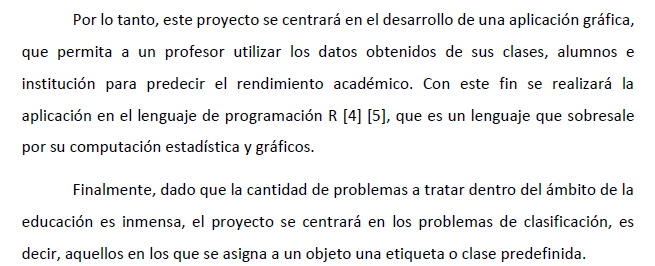
\includegraphics[scale=0.7]{capitulos/img/img2.PNG}
  \caption{Alcance de la idea}
  \label{fig:img2}
\end{figure}

\opinion{Creo que es una buena introducción, contiene elementos introductorios a lo importante del proyecto que son la minería y los entornos educativos, explicando las ideas principales de estas y haciendo fáciles de entender.}

\section{Definición del Problema}

El autor empieza a desarrollar la definición tanto técnica como funcional del problema y todas aquellas especificaciones necesarias para enfrentarse al problema propuesto.

El autor manifiesta de forma precisa que existen dos tipos de secciones en este apartado , el problema real y el técnico.

El autor detalla con exactitud los objetivos
y también redacta el ciclo del mantenimiento de la aplicación junto.

Por último, el autor realiza un resumen de lo que será la definición de los objetivos.

\hspace{15px}

\opinion{Este apartado esta super completo el usuario define perfectamente el problema real del técnico y a la hora de identificar el problema técnico ha usado la \textbf{PDS o (Product Design Specification)} con la que hace un análisis de varias características generales del proyecto a desarrollar, de forma que, con la definición de todas ellas, se consiga una descripción formal del problema técnico.}

\section{Objetivos}

El autor expone el principal objetivo de su proyecto que es: \textbf{El principal objetivo de este proyecto consiste en desarrollar una aplicación gráfica web que permita a un profesor subir datos, visualizarlos y preprocesarlos con el objetivo de entrenar modelos predictivos para problemas de clasificación y predecir nuevos datos que también se subirán a la aplicación}, para ello define los objetivos que debe de cumplir la aplicación, aunque no veo que haya incluido otro tipo de objetivos.

El autor quiere transmitir los objetivos del proyecto para
que una persona no experta pueda entender claramente y sin confusión los objetivos.

\hspace{15px}

\opinion{Este capitulo es muy mejorable, solo se centra en los objetivos principales de la aplicación cuando también debería de incluir los \textbf{objetivos personales y objetivos específicos}, pienso que hizo una mezcla entre los específicos y generales ya que entro en detalle en algunas partes de sus objetivos generales. Con lo cual yo haría tres subsecciones en este apartado que serian las mencionadas: \textbf{Objetivos principales,personales,específicos}}

\section{Antecedentes}

En este apartado se menciona toda aquella información previa que sirve de base para la ejecución del proyecto. Debe prestarse especial atención a comentar y criticar otras aplicaciones existentes en el mercado con utilidades iguales o similares.

El autor únicamente habla de \textbf{R, Shiny,RStudio,Caret},las librerías básicas de uso y poco mas, es muy importante que en este apartado se busquen otros softwares similares o que arrojen la misma luz que el que estamos desarrollando, de esta manera la implantación del nuevo software sería justificable al solventar las carencias o deficiencias de los otros softwares existentes en el mercado y por ello en esta sección es de vital importancia indagar sobre las alternativas en el mercado para luego realizar una comparación y evaluación critica entre ellos.

\hspace{15px}

\opinion{Este capitulo es muy mejorable , me da la sensación que se parece mas a un capitulo de \textbf{recursos software usados} que de antecedentes, en este caso se debería de indagar muchísimo mas en las alternativas que existen en el mercado para justificar que tu estés creando un nuevo software porque incluya mejores elementos, pero en este caso no ha sido así, no ha indagado nada sobre otros elementos software del estilo. No se si la indagación sobre otros software simulares la hará en otro capitulo pero en el capitulo que debe de estar es en este.}

\section{Restricciones}

En este apartado el autor expone todas aquellas restricciones existentes en el ámbito del diseño y que condicionan la elección de una u otra alternativa.

Es importante en lo que respecta al autor, clasificar desde el primer momento las distintas restricciones.

El autor diferencia e identifica los factores dato y estratégicos que es principalmente de lo que tratan las restricciones de un problema real. 

\hspace{15px}

\opinion{El autor cumple bien la definición de ambos factores, espero que haya tenido en cuenta que alguno de los factores datos son inherentes al cliente que este caso habrá sido alguno de los dos profesores que le han llevado el proyecto. 

Pienso que podría haberse metido mas contenido en este apartado aunque de manera general expone bien cuales son ambos factores.}

\section{Recursos}
En este apartado se deben de exponer cuáles son los recursos a utilizar para el desarrollo.

La división básica de recursos debería de contar con:
\begin{enumerate}
    \item \textbf{Recursos humanos: } Jefe de proyecto, los analistas de sistemas, comerciales y técnicos, los programadores, etc.
    \item \textbf{Recursos hardware y software: } Equipos y programas involucrados. 
\end{enumerate}

El autor divide correctamente el apartado de recursos en \textbf{Recursos humanos y recursos materiales(Hardware y software)}, en el apartado de recursos humanos expone quienes son los integrantes y son el propio autor y los dos profesores que llevan el proyecto con el, y en la parte de recursos hardware y software hace un desglose completo y detallado de todos los elementos que serán necesarios para la ejecución del proyecto.

\hspace{15px}

\opinion{Este apartado esta bien estructurado y como lector logras entender cuales son los recursos necesarios para la ejecución del proyecto ya que en este apartado el autor deja de manifiesto perfectamente cuales son todos los elementos tanto humanos y elementos físicos y lógicos necesarios para la ejecución del proyecto, haciéndolo saber al lector mediante diferentes secciones.}

\section{Especificación de requisitos}
En esta sección de un manual técnico se debe incluir y expresar desde el punto de vista técnico, las condiciones obtenidas durante la identificación del problema. Se responderá aquí a las cuestiones mencionadas en la definición del problema técnico. Esta y la siguiente sección del documento son las mas importantes.

El autor expone una breve introducción y hace una división de la especificación en tres subsecciones.
    \begin{enumerate}
        \item \textbf{Especificación de requisitos: } se expondrá de forma detallada los requisitos extraídos de la etapa de definición del problema.
        \item \textbf{Descripción de la información: } se hará una descripción de los datos, la información a tratar y los flujos de datos.
        \item \textbf{Descripción funcional: } se describirán las funciones a implementar para tratar la información de forma adecuada, en función de los requisitos establecidos previamente. Para ello se utilizarán diagramas de casos de uso.
    \end{enumerate}

Toda la información que incluye el autor en esta sección es muy detallada y da con precisión la idea que quiere llevar a cabo.La especificación de requisitos de la aplicación es realmente precisa y también se detalla a buen nivel la estructura de los datos de entrada que requerirá la aplicación así como también nombra elementos como la robustez y la seguridad que son palabras clave a la hora de realizar un proyecto software.

Lo mejor de esta sección son los diagramas de caso de uso que ha incluido mediante UML y als tablas que describen cada CU-XX con los que se puede entender como interactúan los elementos del sistema entre ellos y el propio usuario final ante la aplicación, este seria un ejemplo:

\begin{figure}[H]
  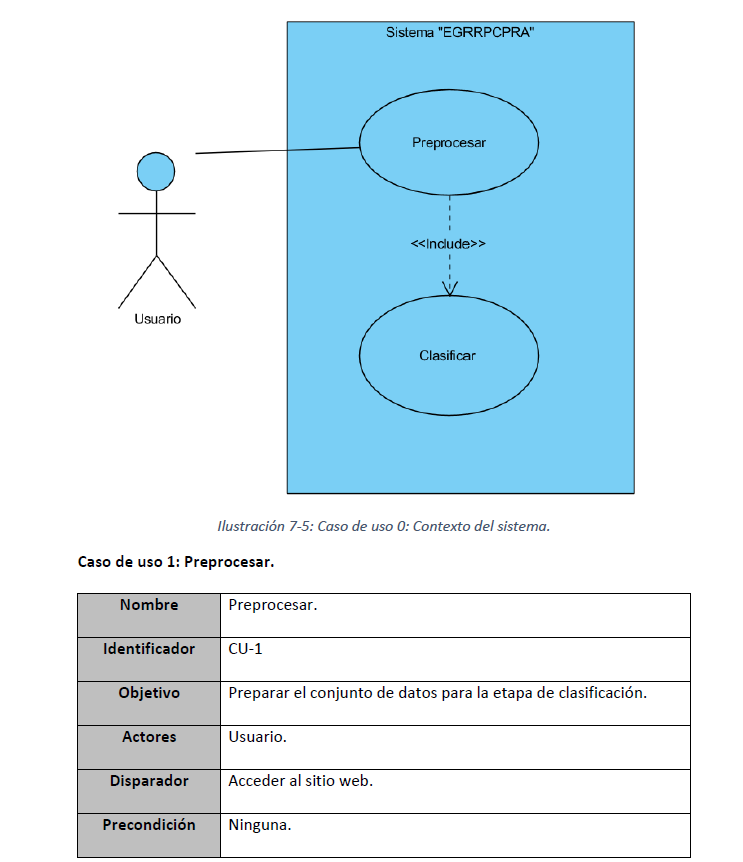
\includegraphics[scale=0.7]{capitulos/img/img3.PNG}
  \caption{Ejemplo caso de uso, CU-1}
  \label{fig:img3}
\end{figure}

\clearpage
\hspace{15px}

\opinion{

Falta algo importantísimo en esta sección, y es que dentro de la especificación de requisitos existen:
    \begin{enumerate}
        \item  \textbf{Requisitos funcionales}
        \item  \textbf{Requisitos no funcionales}
        \item  \textbf{Requisitos de sistema}
        \item  \textbf{Requisitos de usuario}
    \end{enumerate}
    
El autor no ha mencionado en ningún momento esto y es muy importante y necesario identificar cuales son cada uno de los requisitos y en que tipo entrarían.

En esta sección también se deberían de haber hablado de los requisitos lógicos de la aplicación como la estructura de las clases usada en el software y todos los elementos que forman el sistema lógico, esto es muy importante para entender la cohesión y el acoplamiento entre los elementos del software desarrollado.

El autor debería de haber incluido \textbf{la descripción de la información y la adscripción funcional} dentro de la especificación de requisitos y no al mismo nivel creando un poco de confusión.

a favor decir que el autor logra a través de los Casos de uso y de las tablas descriptivas dotar de mucha información al lector sobre las interacciones entre los elementos del sistema.

}

\section{Especificación del Sistema}

Esta sección ha sido llamada por el autor como diseño, esta sección es la ultima parte de la memoria técnica y se centra en la aplicación del diseño a la especificación de requisitos hecha anteriormente. Se detallará en varios apartados el diseño de la interfaz de usuario y el desarrollo final de cada una de las funciones mencionadas en la Especificación de requisitos, explicando su funcionamiento interno. 

Esta secciones debería de tener subsecciones que trataran en las cuales deberían de incluirse:
    \begin{enumerate}
        \item  Diseño de datos.
        \item Diseño arquitectónico.
        \item Diseño procedimental.
        \item Diseño de la interfaz.
    \end{enumerate}

Como hemos comentado en la anterior sección al no haber creado correctamente la estructura para definir los diferentes tipos de requisitos, la estructura de esta sección también esta mal planteada.

El autor da una breve introducción lo cual esta bien y además menciona los tipos de pruebas que hay que son \textbf{ de caja blanca y de caja negra.}

El autor realiza correctamente los dos tipos de prueba que plantea:
    \begin{itemize}
        \item \textbf{Pruebas externas: verificará que cualquiera de las funcionalidades de la aplicación tiene como resultado la salida esperada }
        \item \textbf{Pruebas internas: se encargará de verificar que se ejecutan todos los caminos posibles.}
    \end{itemize}

El autor ha probado cada uno de los casos de uso de la sección anterior creando una tabla de entrada y salida, esta tabla hace referencia al CU-XX y cuales son los efectos de tener una entrada determinada, un ejemplo:

\begin{figure}[H]
  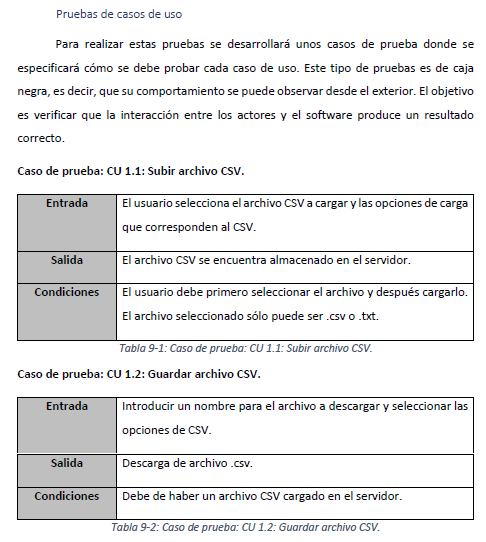
\includegraphics[scale=0.7]{capitulos/img/img4.PNG}
  \caption{Ejemplo caso de prueba}
  \label{fig:img4}
\end{figure}

El autor realiza las pruebas y su estudio mediante unas tablas que comprueba la estabilidad de la prueba realizada, esto es muy importante, un ejemplo:

\begin{figure}[H]
  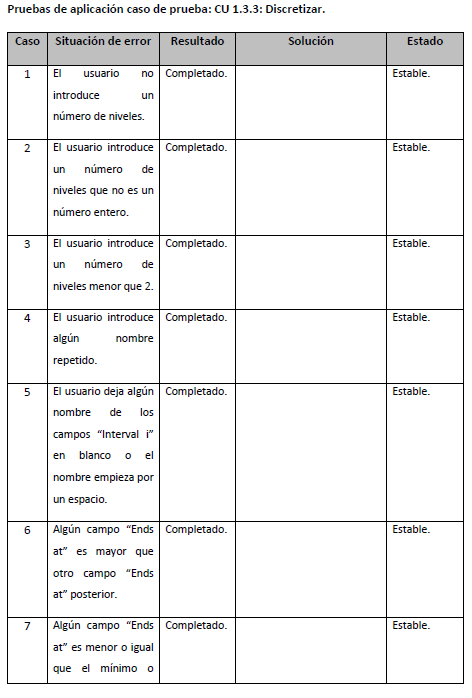
\includegraphics[scale=0.7]{capitulos/img/img5.PNG}
  \caption{Pruebas}
  \label{fig:img5}
\end{figure}
\clearpage
\hspace{15px}

\opinion{

El autor podría haber metido la parte de evaluación de pruebas en esta sección pero ha echo bien en crear una sección aparte para ello.

Se deberían de haber echo las partes del diseño conforme a los diferentes tipos de requisitos que hay y que el autor en la sección anterior no menciono:
    \begin{enumerate}
        \item  \textbf{Requisitos funcionales}
        \item  \textbf{Requisitos no funcionales}
        \item  \textbf{Requisitos de sistema}
        \item  \textbf{Requisitos de usuario}
    \end{enumerate}

Por ello esta sección esta mal estructurada.

Esta sección debería de estar mas desglosada mediante estas subsecciones:

    \begin{enumerate}
        \item  Diseño de datos.
        \item Diseño arquitectónico.
        \item Diseño procedimental.
        \item Diseño de la interfaz.
    \end{enumerate}

La sección de pruebas esta bien planteada y abordada.
}

\section{Conclusiones}

Este apartado, si bien no obligatorio, es de utilidad para ayudar a los técnicos que tengan que mejorar o mantener el software que se presenta. Su objeto es el de poner de manifiesto los puntos débiles y fuertes del software desarrollado y orientar a los futuros desarrolladores sobre las mejoras a implementar.

EL autor expone que ha logrado completar todos los objetivos planteados y que en en la fase de pruebas ha quedado satisfecho con la estabilidad del software desarrollado, también menciona que hay situaciones que no han sido probadas y que pueden fallar que habría que estudiarlas.

\hspace{15px}

\opinion{ 
Yo personalmente habría echo tres partes dentro de esta sección que son:

\begin{itemize}
    \item \textbf{Conclusiones generales de la aplicación}
    \item \textbf{ Futuras mejoras: } Este apartado el autor lo puso aparte
    \item \textbf{Conclusiones personales}
personales
\end{itemize}

EL autor concluye que esta satisfecho con el trabajo realizado.

}

\section{Futuras mejoras}

Aunque la interfaz cumple con los objetivos que el autor planteo al principio,
durante el desarrollo y programación de la misma seguramente se  plantearon nuevos objetivos que aportarían más funcionalidad a la misma, algunos seguramente se habrán cumplido y se han conseguido incorporar a la misma con el resultado que se ha estudiado, pero otros se habrán planteado como futuras mejoras ya que, por diversas causas tales como su dificultad o la falta de tiempo en la realización, el autor no ha podido alcanzar las mismas, y por ello el autor expone en una lista las futuras mejoras.

\hspace{15px}

\opinion{Este apartado podría haberse incluido dentro de la sección anterior, el autor ha sido capaz de identificar las carencias de su sistema y hablar de ellas para en un futuro adquirir tales mejoras.}

\section{Bibliografía}
En esta sección el autor debe listar todas las referencias bibliográficas
utilizadas para la realización del proyecto que aparezcan en el Manual Técnico.

En este caso autor se decanta por una bibliografía numérica, en la que a lo largo de todo el texto podamos ir a la referencia de la misma:
\begin{center}
    \begin{figure}[H]
  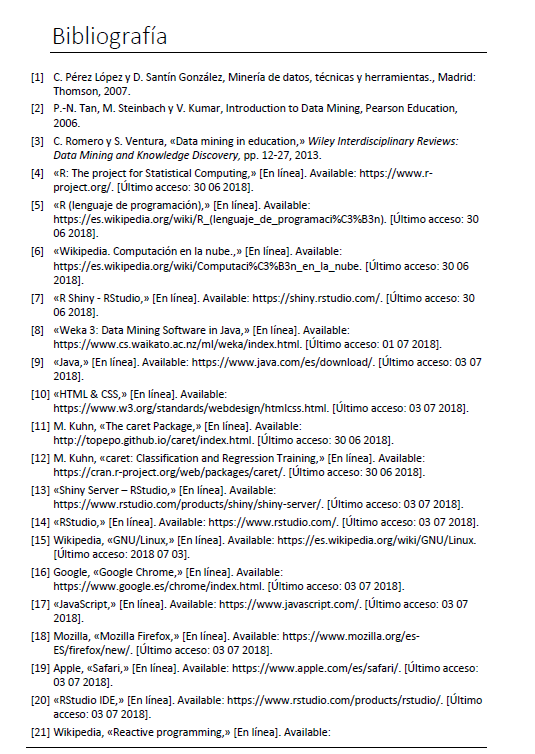
\includegraphics[scale=0.5]{capitulos/img/img6.PNG}
  \caption{Bibliografía}
  \label{fig:img6}
\end{figure}

\end{center}

\opinion{En este apartado no hay mucho que opinar, personalmente me encanta la bibliografía numerada aunque no es muy común, el autor ha citado cada una de las entradas en la bibliografía ene el texto.}


\chapter{Análisis del diseño del documento}

En esta capítulo voy a hablar del manual técnico desde el punto de vista de la presentación y diseño dando así puntos a favor y en contra.

    \begin{enumerate}
        \item \textbf{Puntos a favor: }
            \begin{itemize}
                \item La portada es sencilla e incluye todos los elementos como el titulo, los logos de la universidad, los profesores, grado, especialización todo.
                \item Tablas de figuras y contenidos añadidas al principio.
                \item Ha usado \LaTeX para el manual, con lo cual dota de calidad la memoria técnica.
                \item No he encontrado faltas de ortografía.
                \item Bien estructurado.
                \item Incluye indice de contenidos y de figuras.
            \end{itemize}
        \item \textbf{Puntos en contra: }
            \begin{itemize}
                \item Aunque este bien estructurado de manera general, hay secciones que deberían de ir en otro sitio.
                \item En algunas secciones falta una división mas detallada para comprender mejor las partes.
                \item Se echan en falta elementos gráficos de mejor calidad.
                \item La especificación de requisitos es el apartado mas completo pero peor estructurado.
                \item Falta una sección que hable de la estructura lógica de la propia aplicación.
                \item Echo en falta una figura que explique el modelo de ficheros y estructuras en carpetas que seguirá la aplicación.
                \item Se debería de haber comentado patrones de diseño usados.
                \item No incluye anexos para aprender a usar R ni los otros elementos mencionados.
                \item En el apartado de pruebas se deberían de haber incluido figuras de la aplicación dando los resultados estudiados.
                \item Falta una sección donde se muestre el diseño final de la aplicación.
                \item Hecho en falta un análisis de las pruebas donde un usuario normal sin tantos conocimientos usase la aplicación y generase diferentes tipos de errores y preguntas.
                \item No hay planificación temporal ni nada al respecto.
            \end{itemize}
    \end{enumerate}


\chapter{Conclusiones personales}

En mi opinión el documento requiere de mas mimo por parte del autor, aunque hay secciones que describen a la perfección lo que deben, hay otras que están bastante pobres. Si entrar en profundidad de cada sección, el autor sigue el uso de las secciones siguientes de manera correcta:

\begin{enumerate}
    \item Introducción 
    \item Definición del Problema 
    \item Objetivos 
    \item Antecedentes Otros
    \item Restricciones
    \item Recursos
    \item Especificación de Requisitos
    \item Especificación del Sistema
    \item Conclusiones
    \item Bibliografía
\end{enumerate}

Aunque hay secciones que deberían de reflejar una mejor organización y división dentro de ellas.

Como conclusión final he de admitir que este trabajo me ha servido muchísimo de cara a mi futuro tfg el cual realizare en unos meses, pues he tenido que estudiar e indagar sobre cada sección concienzudamente para comprender que estaba bien que estaba mal y que estaba regular. 

Espero poder aplicar de manera correcta todo lo que he aprendido con esta actividad y que así mi futuro manual técnico sea enriquecido con calidad.